\section{Resultados: coeficientes fijos frente a dinámicos}
\label{sec:resultados_dinamicos}

En esta sección se comparan dos implementaciones de PSO sobre la función F5 (Shifted and Rotated Rastrigin) del benchmark CEC 2017 en 10, 20 y 30 dimensiones. A diferencia de la Sección~\ref{sec:resultados}, en la que solo cambiaba el coeficiente de inercia $w$ y se mantenía $c_1 = c_2 = 1.5$, aquí cambian los tres coeficientes $w$, $c_1$ y $c_2$. La primera implementación usa valores fijos durante toda la ejecución y la segunda los modifica en cada iteración (Tabla~\ref{tab:coeficientes}).

\begin{table}[H]
\centering
\caption{Coeficientes de las dos implementaciones de PSO.}
\label{tab:coeficientes}
\begin{tabular}{lccc}
\toprule
Implementación & $w$ & $c_1$ (cognitivo) & $c_2$ (social) \\
\midrule
PSO fijo & $0.7298$ & $1.49618$ & $1.49618$ \\
PSO dinámico & $0.9 \to 0.4$ & $2.5 \to 0.5$ & $0.5 \to 2.5$ \\
\bottomrule
\end{tabular}
\end{table}

Los valores fijos son los propuestos por Clerc y Kennedy~\cite{clerc2002particle}. En la implementación dinámica los tres coeficientes varían linealmente con la iteración $t$, siguiendo el esquema de coeficientes de aceleración variables en el tiempo (TVAC) de Ratnaweera et al.~\cite{ratnaweera2004self}:
\begin{align}
w(t)   &= w_{max} - (w_{max}-w_{min})\,\frac{t}{T}, \label{eq:tvac_w}\\
c_1(t) &= c_{1i} + (c_{1f}-c_{1i})\,\frac{t}{T}, \label{eq:tvac_c1}\\
c_2(t) &= c_{2i} + (c_{2f}-c_{2i})\,\frac{t}{T}, \label{eq:tvac_c2}
\end{align}
donde $T = 1000$ es el número total de iteraciones. Al inicio domina el componente cognitivo, que favorece la exploración, y al final domina el social, que favorece la explotación alrededor del mejor global.

Cada implementación se ejecutó 30 veces por dimensión con 50 partículas y 1000 iteraciones. Se usaron las mismas semillas que en la Sección~\ref{sec:resultados}, de modo que la ejecución $k$ de ambas implementaciones partió de la misma población inicial. La métrica reportada es el error $f(x_{best}) - f^*$, con $f^* = 500$.

\subsection{Mejor solución, media y desviación estándar}

La Tabla~\ref{tab:fijo_dinamico} presenta, para cada dimensión, la mejor solución encontrada en las 30 ejecuciones, junto con la media y la desviación estándar del error final. El mejor valor de cada dimensión aparece en negritas.

\begin{table}[H]
\centering
\caption{Resultados de PSO con coeficientes fijos y dinámicos en F5 (Rastrigin), 30 ejecuciones.}
\label{tab:fijo_dinamico}
\small
\setlength{\tabcolsep}{4pt}
\begin{tabular}{llcccc}
\toprule
$D$ & Implementación & Mejor $f(x)$ & Mejor error & Media $\pm$ desv. est. & Peor error \\
\midrule
\multirow{2}{*}{10} & PSO fijo & 505.970 & 5.970 & 17.824 $\pm$ 6.720 & 33.415 \\
 & PSO dinámico & \textbf{503.980} & \textbf{3.980} & \textbf{8.884 $\pm$ 3.485} & \textbf{16.914} \\
\midrule
\multirow{2}{*}{20} & PSO fijo & 527.980 & 27.980 & 53.493 $\pm$ 17.778 & 99.493 \\
 & PSO dinámico & \textbf{511.940} & \textbf{11.940} & \textbf{24.343 $\pm$ 8.852} & \textbf{47.758} \\
\midrule
\multirow{2}{*}{30} & PSO fijo & 578.857 & 78.857 & 123.676 $\pm$ 28.868 & 217.894 \\
 & PSO dinámico & \textbf{541.902} & \textbf{41.902} & \textbf{68.677 $\pm$ 17.727} & \textbf{108.084} \\
\bottomrule
\end{tabular}
\end{table}

La implementación dinámica obtuvo mejores resultados en todas las medidas y en las tres dimensiones. Su error medio es aproximadamente la mitad del de la implementación fija: 8.88 frente a 17.82 en $D=10$, 24.34 frente a 53.49 en $D=20$ y 68.68 frente a 123.68 en $D=30$. Su desviación estándar también es menor (3.49, 8.85 y 17.73, frente a 6.72, 17.78 y 28.87), por lo que el resultado depende menos de la población inicial. Incluso la peor ejecución de la versión dinámica en $D=20$ y $D=30$ (47.76 y 108.08) queda por debajo del error medio de la versión fija.

La Figura~\ref{fig:fijo_dinamico} resume ambas implementaciones. A la izquierda se muestra el valor de cada coeficiente a lo largo de la ejecución y a la derecha el error final medio con su desviación estándar.

\begin{figure}[H]
\centering
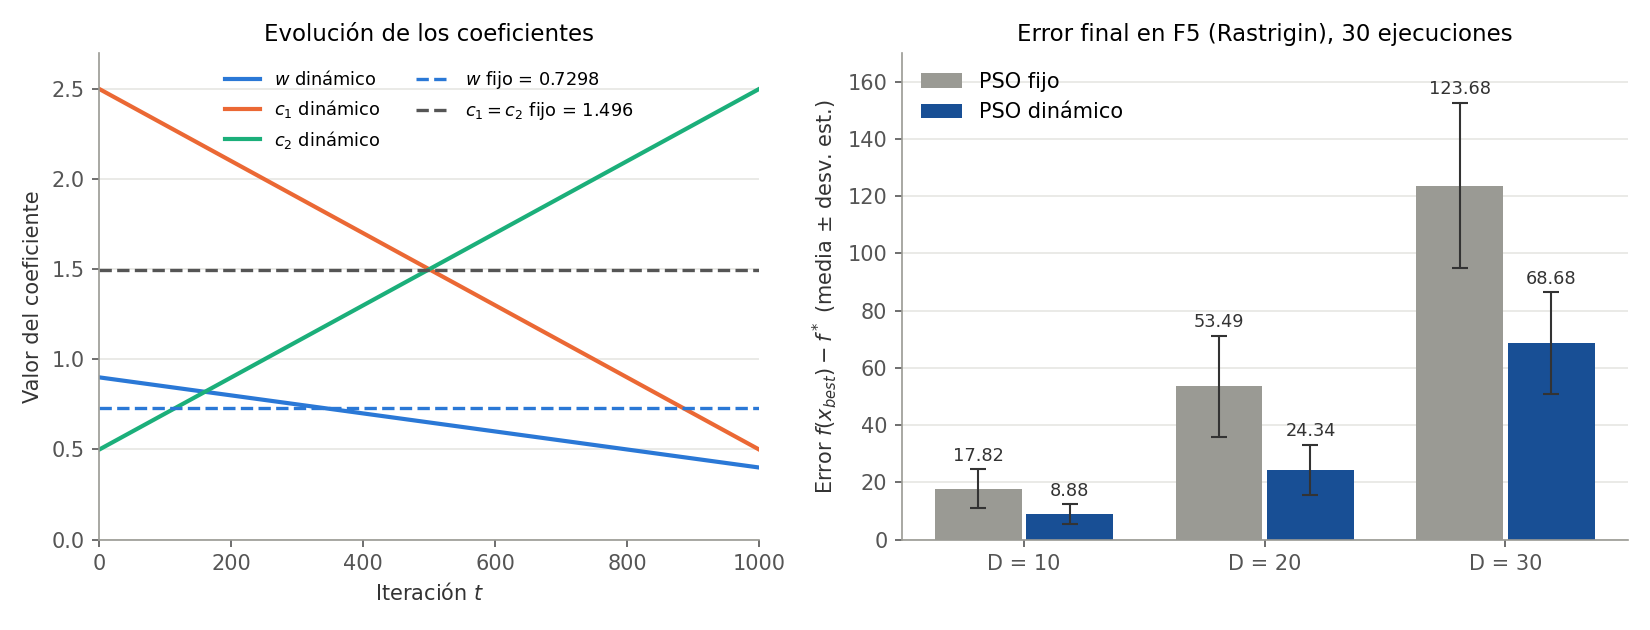
\includegraphics[width=\textwidth]{fijo_vs_dinamico.png}
\caption{Izquierda: valor de $w$, $c_1$ y $c_2$ por iteración (líneas continuas: implementación dinámica; líneas punteadas: implementación fija, donde $c_1$ y $c_2$ coinciden). Derecha: error final medio $\pm$ desviación estándar en 30 ejecuciones para $D = 10$, 20 y 30.}
\label{fig:fijo_dinamico}
\end{figure}

Ninguna ejecución alcanzó el óptimo global. La mejor solución, con $f(x) = 503.98$, se obtuvo con coeficientes dinámicos en $D=10$. Este error de 3.98 es menor que el mínimo registrado en la Sección~\ref{sec:resultados} (4.97, con $w$ lineal y $c_1 = c_2 = 1.5$).

\subsection{Convergencia}

La evolución del error del mejor global durante la ejecución, medida como la mediana de las 30 ejecuciones, explica la diferencia entre ambas implementaciones.


Con coeficientes fijos el error baja rápidamente y después se estanca. La mediana alcanza el 99\,\% de su mejora total alrededor de la iteración 143 en $D=20$ y 186 en $D=30$, y a partir de ahí la curva es prácticamente plana. En $D=20$, por ejemplo, el error mediano es 49.5 tanto en la iteración 200 como en la 1000. El enjambre converge de forma prematura a un mínimo local de Rastrigin.

Con coeficientes dinámicos, las primeras iteraciones son más lentas. En la iteración 200 el error mediano es 27.2 en $D=10$, 110.9 en $D=20$ y 230.7 en $D=30$, mayor que el de la versión fija en las tres dimensiones (19.9, 49.5 y 122.9). En esta etapa $w$ y $c_1$ son altos y $c_2$ es bajo, así que cada partícula explora cerca de su propia trayectoria y la atracción hacia el mejor global es débil. Conforme $c_2$ aumenta y $w$ disminuye, el error baja de forma pronunciada y la curva cruza a la de la versión fija cerca de la iteración 256 en $D=10$, 301 en $D=20$ y 376 en $D=30$. El cruce ocurre más tarde al aumentar la dimensión. La versión dinámica sigue mejorando hasta la iteración 372, 392 y 456, respectivamente, antes de estabilizarse.

\subsection{Pruebas estadísticas}

Como las ejecuciones de ambas implementaciones comparten semilla, se aplicó la prueba de rangos con signo de Wilcoxon para muestras pareadas. Se eligió una prueba no paramétrica porque la prueba de Shapiro--Wilk rechazó la normalidad del error en $D=20$ para ambas implementaciones y en $D=30$ para la versión fija ($\alpha = 0.05$).

\begin{table}[H]
\centering
\caption{Prueba de Wilcoxon pareada entre PSO fijo y PSO dinámico.}
\label{tab:wilcoxon_fijo_dinamico}
\small
\begin{tabular}{lccc}
\toprule
 & $D=10$ & $D=20$ & $D=30$ \\
\midrule
Mediana del error (fijo) & 16.42 & 49.53 & 117.90 \\
Mediana del error (dinámico) & \textbf{8.89} & \textbf{22.88} & \textbf{65.67} \\
Ejecuciones en que gana el dinámico & 27 / 30 & 29 / 30 & 29 / 30 \\
Valor $p$ & $1.80\times10^{-5}$ & $5.59\times10^{-9}$ & $3.73\times10^{-9}$ \\
\bottomrule
\end{tabular}
\end{table}

La diferencia a favor de la implementación dinámica es significativa en las tres dimensiones ($p < 0.001$). Partiendo de la misma población inicial, la versión dinámica terminó con menor error en 27 de las 30 ejecuciones en $D=10$ y en 29 de 30 en $D=20$ y $D=30$.

\subsection{Comparación con los resultados de la Sección~\ref{sec:resultados}}

Como se usaron las mismas semillas, los resultados también pueden compararse de forma pareada con las configuraciones de la Sección~\ref{sec:resultados}. La implementación fija no difiere significativamente de $w = 0.7298$ con $c_1 = c_2 = 1.5$ ($p = 0.349$, 0.584 y 0.855 en $D = 10$, 20 y 30), lo cual es esperable porque sus coeficientes son casi iguales.

La implementación dinámica mejora a la estrategia de $w$ lineal $0.9\to0.4$ con $c_1 = c_2 = 1.5$, que había sido la mejor configuración. El error medio pasa de 14.54 a 8.88 en $D=10$, de 37.76 a 24.34 en $D=20$ y de 82.61 a 68.68 en $D=30$. La diferencia es significativa en $D=10$ y $D=20$ ($p = 3.45\times10^{-5}$ en ambos casos), pero no en $D=30$ ($p = 0.058$), donde la versión dinámica ganó en 21 de las 30 ejecuciones. Como ambas estrategias reducen $w$ de la misma forma, esta mejora se debe a la variación de $c_1$ y $c_2$: dar más peso al componente cognitivo al inicio y al social al final ayuda a evitar la convergencia prematura en Rastrigin.